\documentclass[a4paper]{article}
\usepackage{graphicx}
\usepackage{amsmath}
\usepackage{float}
\usepackage{geometry}
\usepackage{listings}
\usepackage{multicol}
\usepackage{float}
\usepackage{caption}
\usepackage{enumitem}
\usepackage[americanvoltages,fulldiodes,siunitx]{circuitikz}
\usepackage{wrapfig}
\usepackage{mathrsfs} % https://www.ctan.org/pkg/mathrsfs
\newcounter{MyCounter}
\usepackage{enumitem}
\usepackage{pgfplots}
\usepackage{subfig}	% ploting figures beside each other
\pgfplotsset{compat=1.12}

 \geometry{
 a4paper,
 total={170mm,257mm},
 left=20mm,
 top=20mm,
 }
\usepackage{fancyhdr}
\pagestyle{fancy}
\cfoot{(\space \space \space \space \textbf{\thepage}  \space \space \space)}
\renewcommand{\headrulewidth}{1pt}
\renewcommand{\footrulewidth}{1pt}

\usepackage{listings}
\usepackage{color} %red, green, blue, yellow, cyan, magenta, black, white
\definecolor{mygreen}{RGB}{28,172,0} % color values Red, Green, Blue
\definecolor{mylilas}{RGB}{170,55,241}
 
\begin{document}
\lstset{language=Matlab,%
	%basicstyle=\color{red},
	breaklines=true,%
	morekeywords={matlab2tikz},
	keywordstyle=\color{blue},%
	morekeywords=[2]{1}, keywordstyle=[2]{\color{black}},
	identifierstyle=\color{black},%
	stringstyle=\color{mylilas},
	commentstyle=\color{mygreen},%
	showstringspaces=false,%without this there will be a symbol in the places where there is a space
	numbers=left,%
	numberstyle={\tiny \color{black}},% size of the numbers
	numbersep=9pt, % this defines how far the numbers are from the text
	emph=[1]{for,end,break},emphstyle=[1]\color{blue}, %some words to emphasise
	%emph=[2]{word1,word2}, emphstyle=[2]{style},    
}





	\begin{center}
	\textbf{
	\\In the name of God
		}\\
	
	\vspace{2cm}
	\includegraphics[scale=.35]{logo1.png}\\
	\vspace{0.5cm}
	\begin{Large}
	\textbf{
	\\Sharif University of Technology
	\vspace{0.5cm}
	\\School of Electrical Engineering
	}
	\end{Large}
	\vspace{2cm}
	\begin{huge}
	\textbf{
	\\Convex Optimization
	\vspace{0.75cm}
‍
	\\HW Nr. 4, MATLAB
	}
	\end{huge}
	\vspace{2cm}
	\begin{Large}
	\textbf{
	\\Dr. Babazadeh
	\vspace{2cm}
	\\Taha Entesari
	\vspace{0.75cm}
	\\95101117
	}
	\end{Large}
	
\end{center}

\thispagestyle{empty}
\newpage
\begin{Large}
	I was unable to type parts a to c of this homework due to numerous tasks and have sent beside this file the scanned version.
The required code is available in the appendix of this pdf file. The \texttt{.m} file is also available in the folder should you want to run the code for yourself.\\
A sample run of the code results in the following plot:
\begin{figure}[h!]
	\begin{center}
		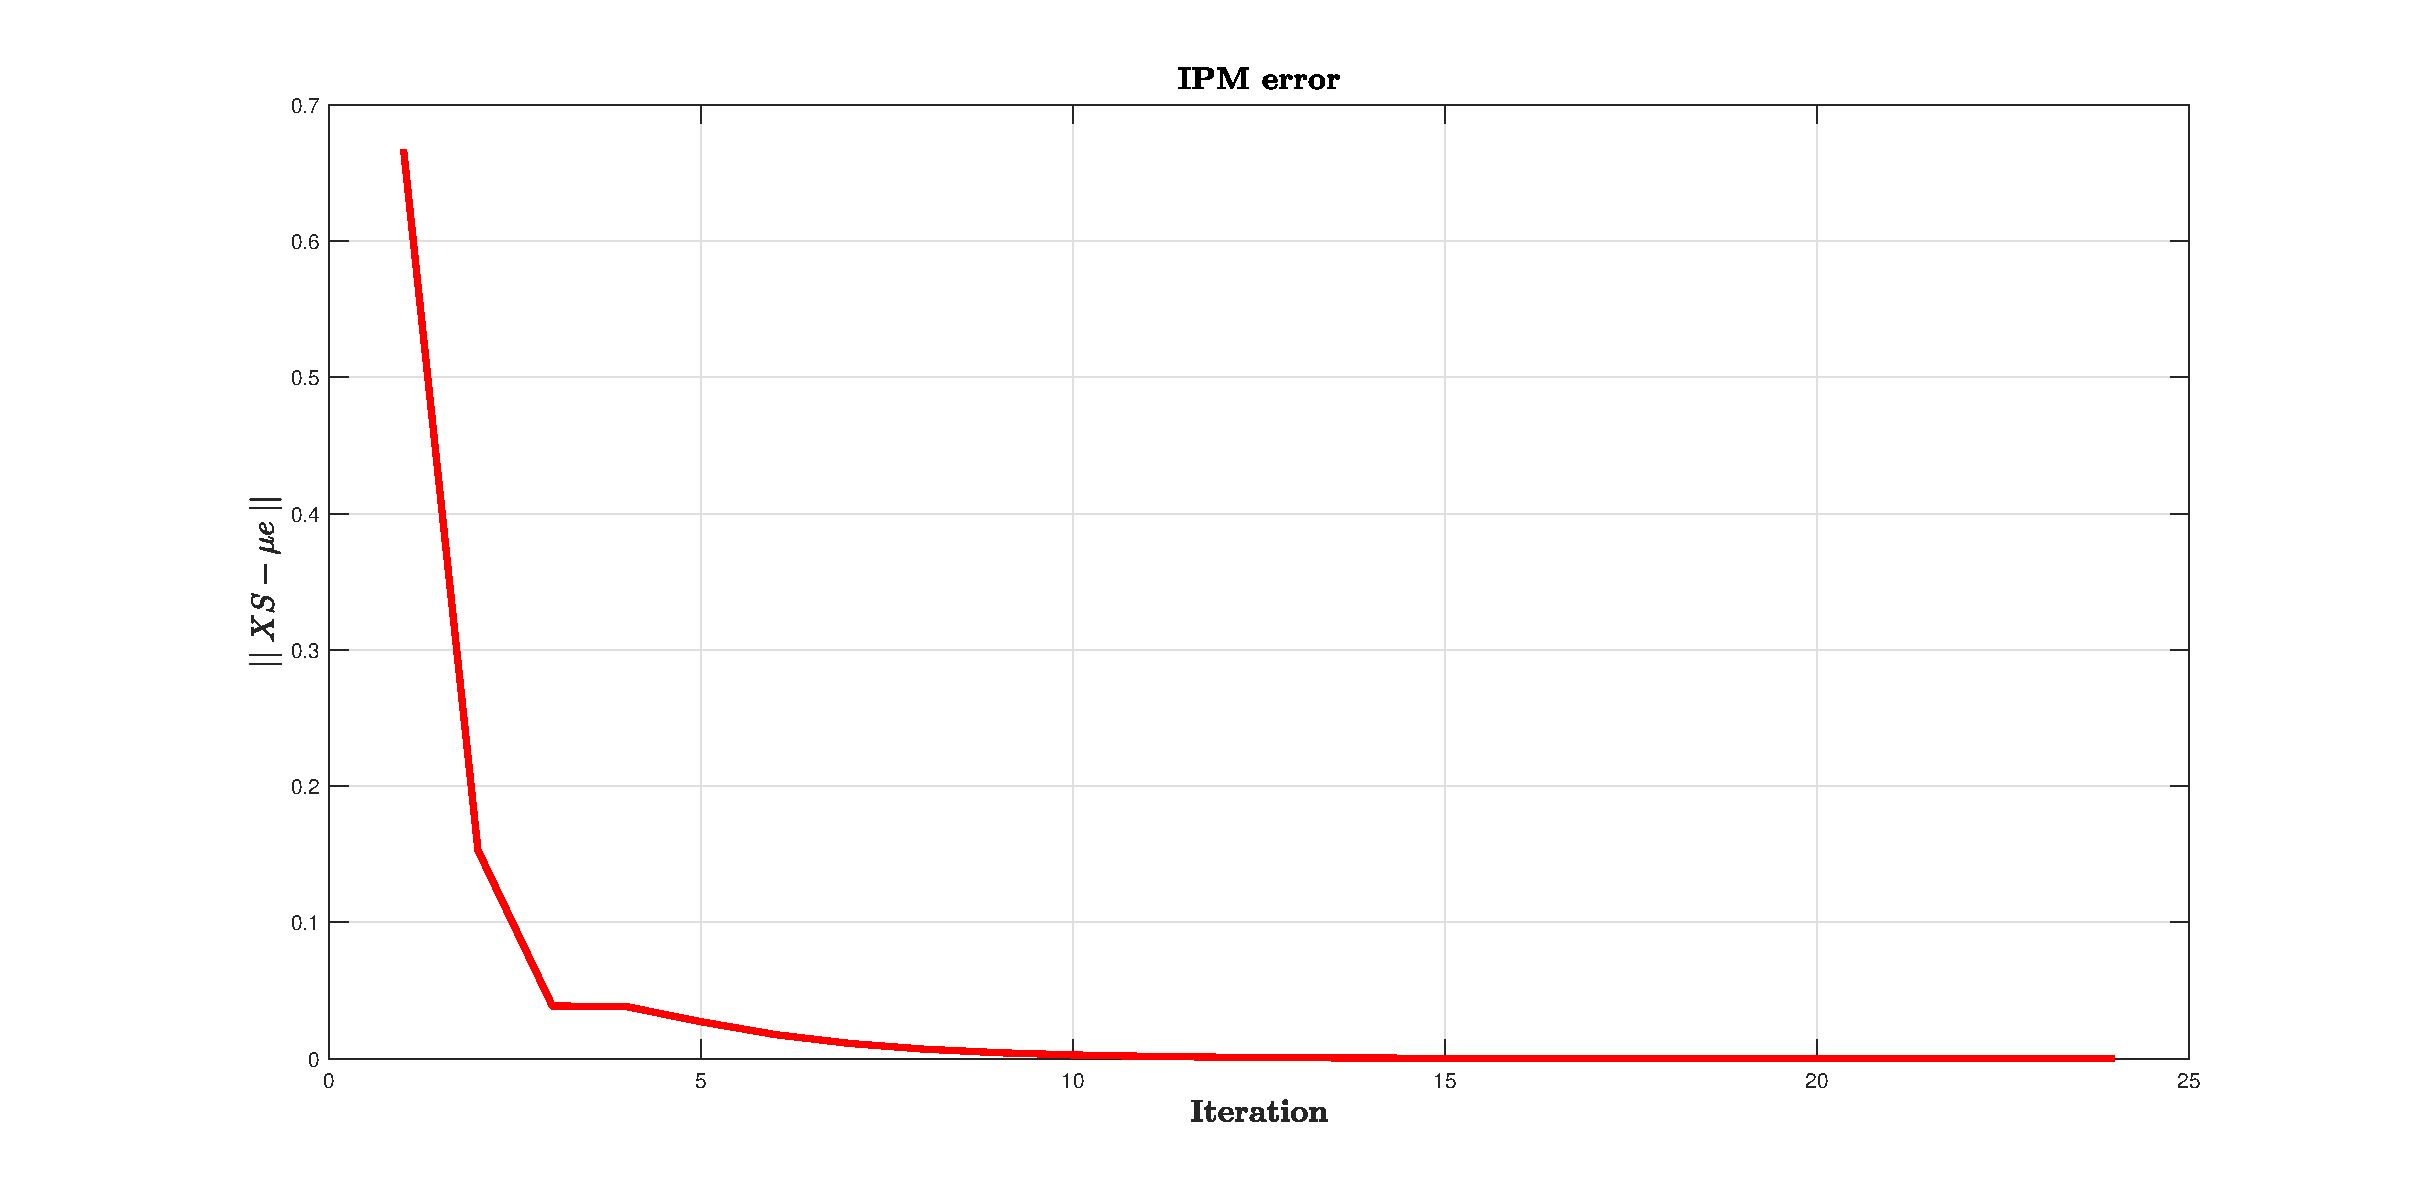
\includegraphics[scale=.45]{error}
	\end{center}
\end{figure}
Having run the code several times I noticed that there also existed cases in which though CVX resulted in a bounded finite optimum value, the implemented method would diverge, But these may be extreme cases with matrices that might be very close to being singular.
\end{Large}
\section*{Appendix: MATLAB Code}
\lstinputlisting{HW4_95101117.m}
\end{document}

